\documentclass[fleqn,10pt]{wlscirep}
\usepackage[utf8]{inputenc}
\usepackage[T1]{fontenc}
\usepackage{lineno}
\linenumbers

\title{Characterisation of space in Great Britain using the Spatial Signatures model}

\author[1, *]{Martin Fleischmann}
\author[1]{Daniel Arribas-Bel}
\affil[1]{Geographic Data Science Lab, Department of Geography and Planning, University
of Liverpool, Roxby Building , 74 Bedford St S , Liverpool , L69 7ZT, United Kingdom}

\affil[*]{corresponding author(s): Martin Fleischmann (m.fleischmann@liverpool.ac.uk)}


\begin{abstract}
This is a manuscript template for Data Descriptor submissions to \emph{Scientific Data}
(\href{http://www.nature.com/scientificdata}{http://www.nature.com/scientificdata}). The
abstract must be no longer than 170 words, and should succinctly describe the study, the
assay(s) performed, the resulting data, and the reuse potential, but should not make any
claims regarding new scientific findings. No references are allowed in this section.
\end{abstract}
\begin{document}

\flushbottom
\maketitle
%  Click the title above to edit the author information and abstract

\thispagestyle{empty}

\noindent Please note: Abbreviations should be introduced at the first mention in the
main text – no abbreviations lists or tables should be included. Structure of the main
text is provided below.

\section*{Background \& Summary}

(700 words maximum) An overview of the study design, the assay(s) performed, and the
created data, including any background information needed to put this study in the
context of previous work and the literature. The section should also briefly outline the
broader goals that motivated the creation of this dataset and the potential reuse value.
We also encourage authors to include a figure that provides a schematic overview of the
study and assay(s) design. The Background \& Summary should not include subheadings.
This section and the other main body sections of the manuscript should include citations
to the literature as needed.

% This section should provide an overview of the study that generated the data, as well as outlining the potential reuse value of the data. Any previous publications that used these data, in whole or in part, should be cited and briefly summarized.

% + Form vs function in classification & missing link
% + detailed x scalable x consistent
% + *largely rephrase main arguments from conceptual paper*
% + summary - spsig in the whole GB
%     - classification and description of space


% Form & Function in cities and their value
How the building blocks that make up cities are spatially arranged is worth
quantifying and understanding.
%% What FF is
By "building blocks", we mean both the activities and agents that inhabit
cities, as well as the (infra)structure that supports them. The
former can be conceptualised as \textit{urban function}, while the latter
falls under the study of \textit{urban form}.
%% Why:
Understanding urban form and function is important for two main reasons.
%%% encodes
First, the combination of both \textit{encodes} much information about the
history, character and evolution of cities.
%
For example, the shape and properties of the street network encode the technology of the
time (e.g., automobile); while the degree of mix in land uses can reflect
cultural values.
%%% influences
Second, the spatial pattern of urban form and function also acts as a
frame that \textit{influences} a variety of outcomes, from economic
productivity to socio-economic cohesion to environmental sustainability.

% We use the Spatial Signatures
In this paper, we use the Spatial Signatures framework \cite{dab_mf_2021a, dab_mf_2021b},
which develops a ``characterisation of space based on form and function
designed to understand urban environments''\cite{dab_mf_2021a}.
%% Signature definition
Spatial Signatures are theory-informed, data-driven computable classes that
describe the form and function of a consistent patch of geography.
%
Figure \ref{fig:workflow} presents an overview of the development of a spatial
signature classification.
%
We build a series of enclosures that we combine with building footprints
to further subdivide geographical space. We then attach form and function
characters to each of these subdivisions, and use those to group them into
consistent and differentiated classes we call signatures.
%
Each phase is expanded in detail in the next section.

\begin{figure}
        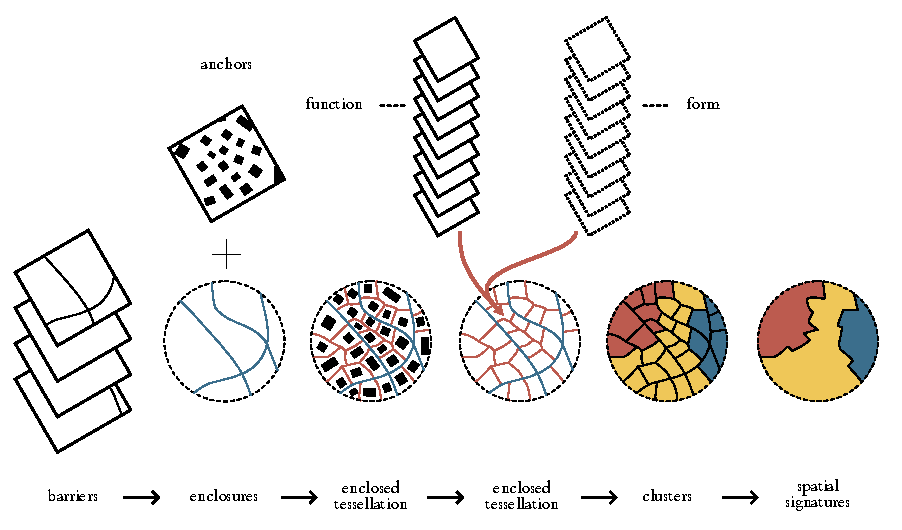
\includegraphics[width=\linewidth]{fig/workflow.pdf}
\caption{Diagram illustrating the sequential steps leading to the delineation of
spatial signatures. From a series of enclosing components, to enclosures,
enclosed tessellation (ET), the addition of form and function characters to ET
cells, and the development of spatial signatures.}
\label{fig:workflow}
\end{figure}

    % In this paper
% Great British Signatures
We introduce an open data product (ODP \cite{odp_paper21}) containing a classification of
spatial signatures for Great Britain. In doing so, we provide an
analysis-ready layer that brings urban form and function consistently, in
detail, and at national scale. To the best of our knowledge, this is the first
dataset capturing urban form and function published both with a degree of detail and scale as
ours.
%% Input data used
Our results are based on the analysis of more than 14 million of ET cells, to
each of which we attach more than 300 characters capturing a wide range of
aspects relating to urban form and function.
%% Data available
We provide access to both granular geographical boundaries of the delineated spatial signatures
as well as measurements for each character at the signature level.
%% Web map and code
The ODP also includes a web map that allows exploration without any technical
requirement other than a web browser, and we have open sourced all the code,
including details on the computational backend.
%% Comparison with other datasets
The uniqueness of our ODP makes setting up a technical validation as a
comparison with existing datasets challenging. Nevertheless, we relate our
signatures to a few well-established data products that capture each a subset
of the form and function dimensions we consider. Our results are encouraging
in that they show broad agreement in expected areas, but also highlight
aspects that can only be discovered when considering form and function in tandem.

% Benefits of signature approach (goals why we created it)
The approach and outputs presented bring several benefits to a range of
stakeholders interested in cities.
%% ODP
This spatial signatures ODP provides insight generated from detailed,
comprehensive and computationally intensive data analysis and presents it in a
way that is easy to access, work with and integrate into larger projects.
%
%%% Academics and policymakers
Together with the importance of form and function discussed above, we
anticipate the output will be relevant to both academic researchers as well as
policymakers and practitioners.
%% Broader SS benefits
As a conceptual framework, the spatial signatures provide a flexible yet
generalisable approach to understand, characterise and quantify urban form and
function. One way to understand our results is as an implementation of a
more general way of thinking about the spatial dimension of cities. In this
context, it can be useful to researchers and practitioners who, even if not
specifically interested in Great Britain, would like to implement a similar
approach.
%
In this respect, we hope the present paper serves not only to document our own
work but to inspire future efforts aimed at urban form and function.



            %%% FROM ORIGNAL GUIDELINE %%%

% An overview of the study design, the assay(s) performed, and the created data, including any background information needed to put this study in the context of previous work and the literature.

%- Briefly outline the broader goals that motivated the creation of this dataset and the potential reuse value.

%- We also encourage authors to include a figure that provides a schematic overview of the study and assay(s) design.




\section*{Methods}

% conceptualisation of signature detection
    % small unit
    % complex descirption (F&F)
    % cluster analysis
The method of identification of spatial signatures consists of three top level steps.
First, we need to delineate spatial unit of analysis, one that reflects the structure of
urban phenomena on a very granular level. Then we charactercterise each of them
according to the form and function capturing the nature of each unit and its spatial
context. Finally, we use cluster analysis to derive a typology of our spatial units
that, once combined into contiguous areas, forms a typology of spatial signatures.

\subsection*{Spatial unit}
% spatial unit
    % conceptualisation of enclosed tessellation
    % rules
        % indivisible
        % internally consistent
        % geographically exhaustive
    % options
        % admin boundaries
        % arbitrary grids
        % morphological units
    % ET design
        % barriers
        % enclosures
        % anchors
        % ET cells
The first major methodological decision needs to be taken on the definition of the
spatial unit. As mentioned, it needs to reflect space in a granular manner and we argue
that it should fulfil three conditions. First, it should be \textit{indivisible},
meaning that when such a unit would be subdivided into smaller parts, none of them would
be enough to capture the nature of spatial signature. Second, it needs to be
\textit{internally consistent} - it should always reflect only a single signature type.
Last, it should be geographically \textit{exhaustive}, covering entirety of the study
area.

Spatial units used in literature can be split into three groups. One is using
administrative boundaries like city regions, wards or census output areas, that are
convenient to obatain and can be easily linked to auxiliarry data. However,
those rarely reflect the morphological composition of urban space and in some cases may
even “obscure morphologic reality” REF Taubenbock 2019. At the same time, most of them
are divisible and larger units are not alwyas internally consistent. Another group is based on
arbitrary uniform grids linked either to spatial indexing method like H3 REF or OS
National Grid REF, or to anciliarry data of remote sensing or other origins like a
WorldPop grid REF. The issue is that grids cannot be considered internally consistent as
they have no relation to the real-life spatial pattern. Finally, urban morphology tends to use morphological elements as
street segments REF, blocks REF buildings or plots as a unit of analysis. Some of those
could be seen as indivisible and internally consistent but since they are largely based
on built-up fabric, they are not exhaustive. When there is no builiding or street, there
is no spatial unit to work with. Plots could be theoretically considered as exhaustive,
consistent and indivisible but there is no accepted conceptual definition and unified
geometric representation (REF Kropf).

We are, therefore, proposing an application of an alternative spatial unit called \textit{enclosed
tessellation cell} (ETC), defined as:

\newtheorem*{theorem}{}
\begin{theorem}
    A characterisation of space based on form and function designed to understand urban
environments
\end{theorem}

% We should drop a reference to conceptual paper here.

ETC follows the morphological tradition in a sense that is it
based on the physical elements of an enviroment but overcomes the drawbacks of
conventionally used units. Its geometry is generated in three steps illustrated on a
Figure \ref{fig:et_diagram}. First, a set of features representing physical barriers
subdividing space, in our case composed of street network, railways, rivers and a
coastline, is combined together, generating a layer of boundaries. These then partition space
into smaller enclosed geometries called \textit{enclosures}, which can be very granular
or very coarse depending on the geographic context. In dense city centres where a single
enclosure represent a single block is a high frequency of small enclosures, while in the
countryside, we can observe very few large enclosures as their delimiters are far away
from each other. Enclosures are then combined with building footprints, posing as
anchors in the space and are subdivided into enclosed tessellation cells using the
morphological tessellation algorithm REF, a polygon-based adaptation of Voronoi
tessellation. Resulting geometries are indivisible as they contain, at most, a single
achor building, internally consistent due to their granularity and link to morphological
elements composing urban fabric, and geogrpahically exhasutive as they cover entire area
limited by specified boundaries.

    % data input
        % barries
            % roads from OS Open Roads
                % data description (simplified centerlines)
            % railway from OS OpenMap - Local
                % data description (simplified centerlines)
            % rivers from OS OpenRivers
                % data description (simplified centerlines)
            % coastline from OS Strategi®
                % data description (continuous enclosing geometry)
        % buildings
            % OS OpenMap - Local
            % data quality description (merged adjacent geometries)

In the case of classification of Great Britain, street networks are extracted from OS
Open Roads datasets (REF) representing simplified road centrelines cleaned of road
segments under the ground. Railways are retrieved from OS OpenMap - Local
("RailwayTrack" layer) which captures surfance railway tracks. Rivers are extracted from
OS OpenRivers (REF) representing river network of GB as centrelines, and a coastline is
retrieved from OS Strategi® (2016) REF, capturing  coastline as a continous line
geometry. Building geometry is extracted, again, from OS OpenMap - Local ("Building"
layer) and represents generalised building footprint polygons. Note that the dataset
does not distinguish between individual buildings when they are adajcent (e.g. perimeter
block composed of multiple buildings is represent by a single polygon).

% characterisation of space
    % form
        % input data
            % ET cells
            % bulidings
            % street network
        % morphometrics
            % different categories of characters
                % dimension
                % shape
                % spatial distribution
                % intensity
                % connectivity
                % diversity
            % different scales
                % individual elements -> adjacency -> networks
        % contextualisation
            % interest in characterisation of spatial patterns
            % distance-weighted higher order contiguity spatial weights
            % reflection of a statistical distribution of data within context
                % proxy of diversity

    % function
        % input data
            % overview - from population and POIs to NDVI and night lights
            % include table with transfer methods
        % transfer methods overview
            % spatial join
            % interpolation
            % accessibility
        % contextualisation
            % depending on the transfer method, function-based characters we
            %  contextualised using the same method used in morphometrics

% cluster analysis
    % comparison of clustering methods (shall we include this?? skip for now)
        % K-Means, GMM, SOM

    % two levels of K-Means clustering
        % data input
            % combination of both form and function, all characters equally weighted
            % only contextualised representation of characters is used to capture pattern

            % data standardisation
                % column-based mean standardisation

        % selection of number of clusters
            % clustergram
            % supplementary metrics
                % Silhouette
                % Calinski-Harabasz
                % Davies-Boulding

        % top level providing a first national classification
        % sub clustering of urban areas
            % selection criteria for to-be-subclustered classes

% generation of signature geometry
    % dissolution based on contiguity and assigned class


% - Feature importance - should this actually be included in here?

\section*{Data Records}

The Data Records section should be used to explain each data record associated with this
work, including the repository where this information is stored, and to provide an
overview of the data files and their formats. Each external data record should be cited
numerically in the text of this section, for example \cite{Hao:gidmaps:2014}, and
included in the main reference list as described below. A data citation should also be
placed in the subsection of the Methods containing the data-collection or analytical
procedure(s) used to derive the corresponding record. Providing a direct link to the
dataset may also be helpful to readers
(\hyperlink{https://doi.org/10.6084/m9.figshare.853801}{https://doi.org/10.6084/m9.figshare.853801}).

Tables should be used to support the data records, and should clearly indicate the
samples and subjects (study inputs), their provenance, and the experimental
manipulations performed on each (please see 'Tables' below). They should also specify
the data output resulting from each data-collection or analytical step, should these
form part of the archived record.

%  This section should be used to explain each data record associated with this work,
%  including the repository where this information is stored, and to provide an overview
%  of the data files and their formats. Each external data record should be cited using
%  our data citation format.

% description of the GPKG/archive
The data product described in this article is available through the Consumer Data
Research Centre Open Data repository available at
\hyperlink{https://data.cdrc.ac.uk/dataset/xxx-xxx-xxx}{https://data.cdrc.ac.uk/dataset/xxx-xxx-xxx}
under the Open Government Licence v3.0 license. The dataset stored in the repository
contains a GeoPackage with a signature geometry (OSGB36 / British National Grid
(\texttt{EPSG:27700}) CRS) and related signature type, plain-text pen portraits describing individual
signature types, a series of CSV files describing individual signatures and signature
types, and a CSV files linking signature types to the Output Area and Lower
Super Output Area geometry. An online interactive map
of spatial signatures for the whole of Great Britain is available on the project website
(\hyperlink{https://urbangrammarai.xyz/great-britain}{https://urbangrammarai.xyz/great-britain}).


\section*{Technical Validation}

This section presents any experiments or analyses that are needed to support the
technical quality of the dataset. This section may be supported by figures and tables,
as needed. This is a required section; authors must present information justifying the
reliability of their data.

Spatial signatures are unique as a classification method, limiting the potential
validation approaches. In this context, we focus on indirect methods that use ancillary datasets capturing
conceptually similar aspects of the environment. We compare the signatures with three of
such datasets, each focusing on a different classification perspective, but all related
to our classification to a degree when we can assume there will be a measurable level of
association between the two:

\begin{itemize}
    \item WorldPop settlement patterns of building footprints (2021)\cite{jochem2021tools}
    \item Classification of Multidimensional Open Data of Urban Morphology (MODUM) (2015)\cite{alexiou2016}
    \item Copernicus Urban Atlas (2018)\cite{eea2018}
\end{itemize}


\subsection*{Validation approach}
% General method of validation
    % data transfer (one or the other way depending on feasibility) chi-squared
    % statistic Cramer's V
All datasets, spatial signatures and those selected as validation contain a
categorical classification of space linked to their unique geometry. The first
requirement to be able to compare data products is to transfer their
information to the same geometry. We take two approaches for this step,
depending on the dataset we are comparing the signatures with:
an interpolation of one set of polygon-based data to another (input to ETCs);
or the conversion of
spatial signatures to the raster representation matching an input raster,
which is computationally more efficient when one of the layers is already a raster. The second
step is a statistical comparison of two sets of classification labels, one representing
spatial signature typology and the other validation classes. We use contingency tables
and Pearson's $\chi^{2}$ test to determine whether the frequencies of observed
(signature types) and expected (validation types) labels significantly differ in one or
more categories. Furthermore, we use Cramér's $V$ statistics\cite{cramer2016mathematical} to assess the strength of
the association.

\subsection*{WorldPop settlement patterns of building footprints}
% - WorldPop (Spsig)
    % description of dataset + figure
WorldPop settlement patterns of building footprints aim to derive a typology of
morphological patterns based on a gridded approach with cells of
100x100m, and building footprints. Authors measure six morphometric characters
linked to the grid cells and use them as input for an unsupervised clustering
algorithm leading to a six-class typology.
    % expectations regarding similarity
As the classification is dependent on building footprints, grid cells that do
not contain any information on the building-based pattern are treated as missing in the
final data product. For the validation of spatial signatures, this \textit{missing}
category is treated as a single class. It is assumed that the top-level large scale
patterns detected by the WorldPop method and spatial signatures will provide similar
results. However, there will be differences caused by the inclusion of function in spatial
signatures, higher granularity of both initial spatial units and the resulting
classification (6 vs 19 classes).

Signature typology is rasterized and linked to the WorldPop grid. The resulting
contingency table is shown in Figure \ref{fig:crosstab_worldpop}. There is a significant relationship between
two typologies, $\chi^{2} (114, N = 22993921) = 13341832, p < .001$. The strength of
association measured as Cram\'{e}r's $V$ is $0.311$, indicating moderate association.
    % results + contingency table figure

\begin{figure}
    \centering
    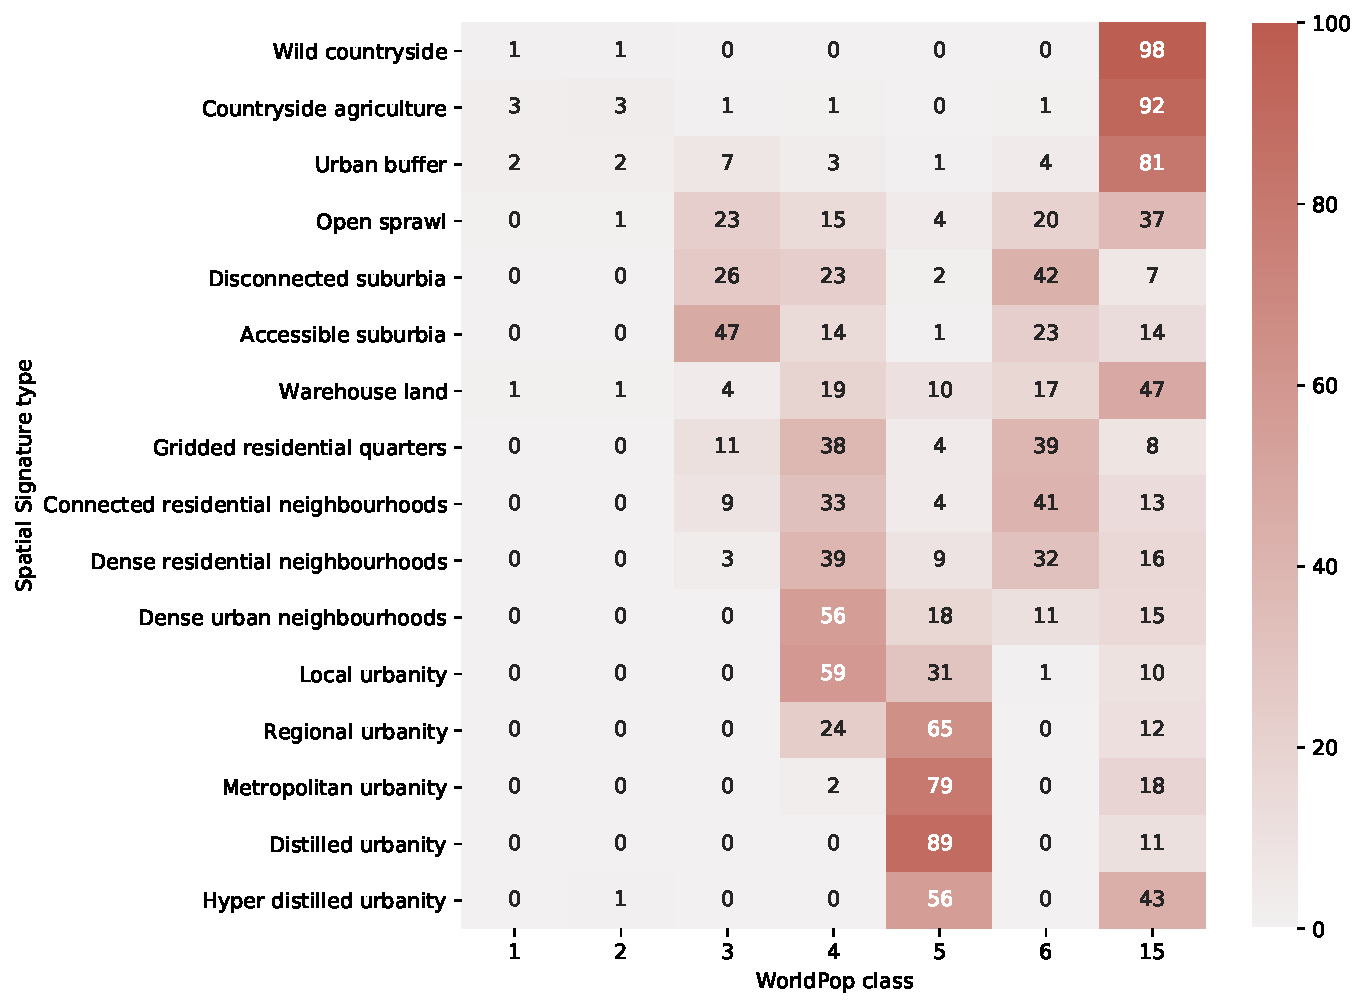
\includegraphics[width=.8\linewidth]{fig/crosstab_worldpop.pdf}
    \caption{Contingency table showing frequencies (in \%) of WorldPop classes within signature types.}
    \label{fig:crosstab_worldpop}
\end{figure}

\subsection*{MODUM}
% - MODUM (Spsig)
    % description of dataset + figure
Multidimensional Open Data Urban Morphology (MODUM) classification describes a typology
of neighbourhoods derived from 18 indicators capturing built environment as streets,
railways or parks, linked to the Census Output Area geometry. The classification
identifies 8 types of neighbourhoods.
    % expectations regarding similarity
Compared to the WorldPop classification, MODUM takes into account more features of
the built environment than building footprints, which makes it conceptually closer to the
spatial signatures. However, it is still focusing predominantly on the form component,
although there are some indicators that would be classified as function within the
signatures framework (e.g. population). The MODUM method uses a different way of
capturing context compared to the signatures, which leads to some classes being
determined predominantly by a single character. For example, the \textit{Railway Buzz} type
forms a narrow strip around the railway network, which is an effect signatures avoid.
    % results + contingency table figure
MODUM typology is available only for England and Wales. Therefore the validation takes
into account only ETCs covering the same area. The classification is linked to the
ETC geometry is based on the proportion (the type covering the largest portion of ETC is
assigned). The resulting contingency table is shown in Figure \ref{fig:crosstab_modum}. There is a
significant relationship between two typologies, $\chi^{2} (152, N = 13067584) =
13938867, p < .001$. The strength of association measured as Cramér's $V$ is $0.300$,
indicating moderate association of very similar levels we have seen above.

\begin{figure}
    \centering
    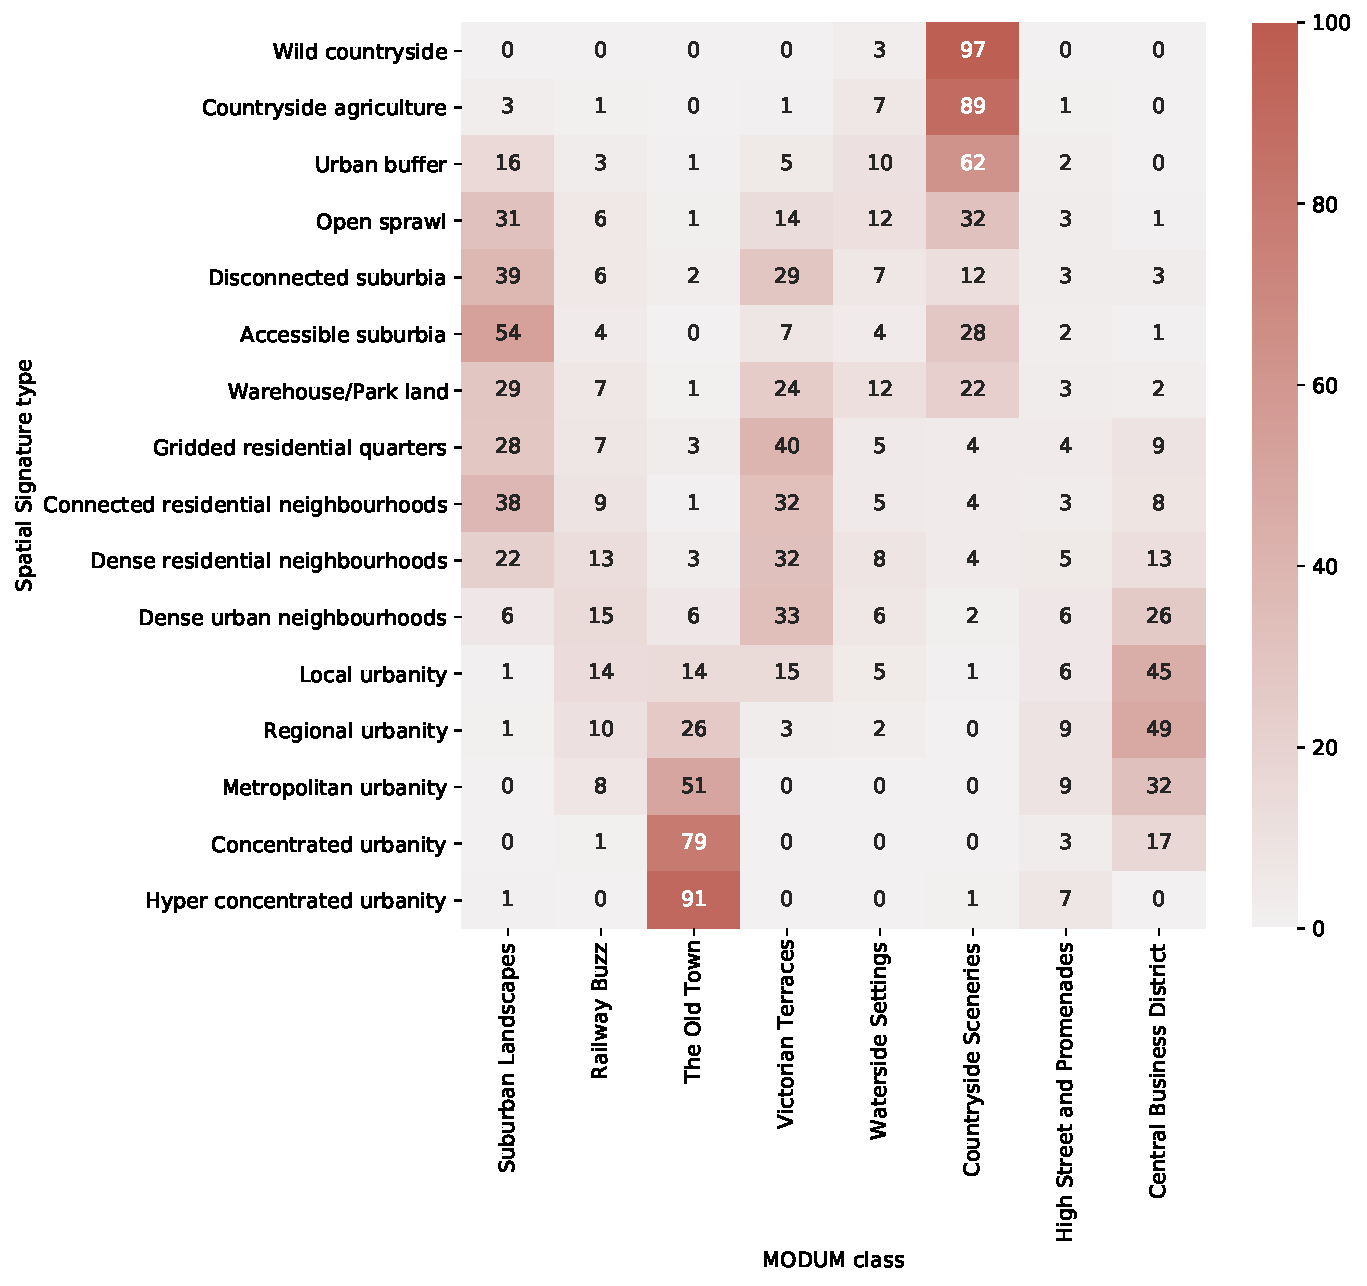
\includegraphics[width=.8\linewidth]{fig/crosstab_modum.pdf}
    \caption{Contingency table showing frequencies (in \%) of MODUM classes within signature types.}
    \label{fig:crosstab_modum}
\end{figure}

\subsection*{Copernicus Urban Atlas}
% - Urban atlas (Spsig)
    % description of dataset + figure
Copernicus Urban Atlas is the least similar of the validation datasets. It is a
high-resolution land use classification of functional urban areas derived primarily from
Earth Observation data enriched by other reference data as OpenStreetMap or topographic
maps. Its smallest spatial unit in urban areas is 0.25 ha and 1 ha in rural areas,
defined primarily by physical barriers. The Urban Atlas classification, which identifies
27 classes predefined classes using the supervised method.
    % expectations regarding similarity
The majority of urban areas is classified as urban fabric further distinguished based on
continuity and density resulting in six classes of the urban fabric. The classification does
not consider the type of the pattern or any other aspect. Furthermore, it does not take
into account what signatures call \textit{context} as each spatial unit is
classified independently, which in some cases leads to the high heterogeneity of
classification within a small portion of land. Signatures take a different approach.
Consequently, it is expected that the similarity between the two will be limited.
    % results + contingency table figure
Urban Atlas is available only for functional urban areas (FUA), leaving rural areas
unclassified. Validation then applies to FUAs only. The classification is linked to the
ETC geometry based on the proportion (the type covering the largest portion of ETC is
assigned). The resulting contingency table is shown in Figure \ref{fig:crosstab_ua}. There is a
significant relationship between two typologies, $\chi^{2} (450, N = 8396642) = 5229900,
p < .001$. The strength of association measured as Cramér's $V$ is $0.186$, indicating
a weak association.

\begin{figure}
    \centering
    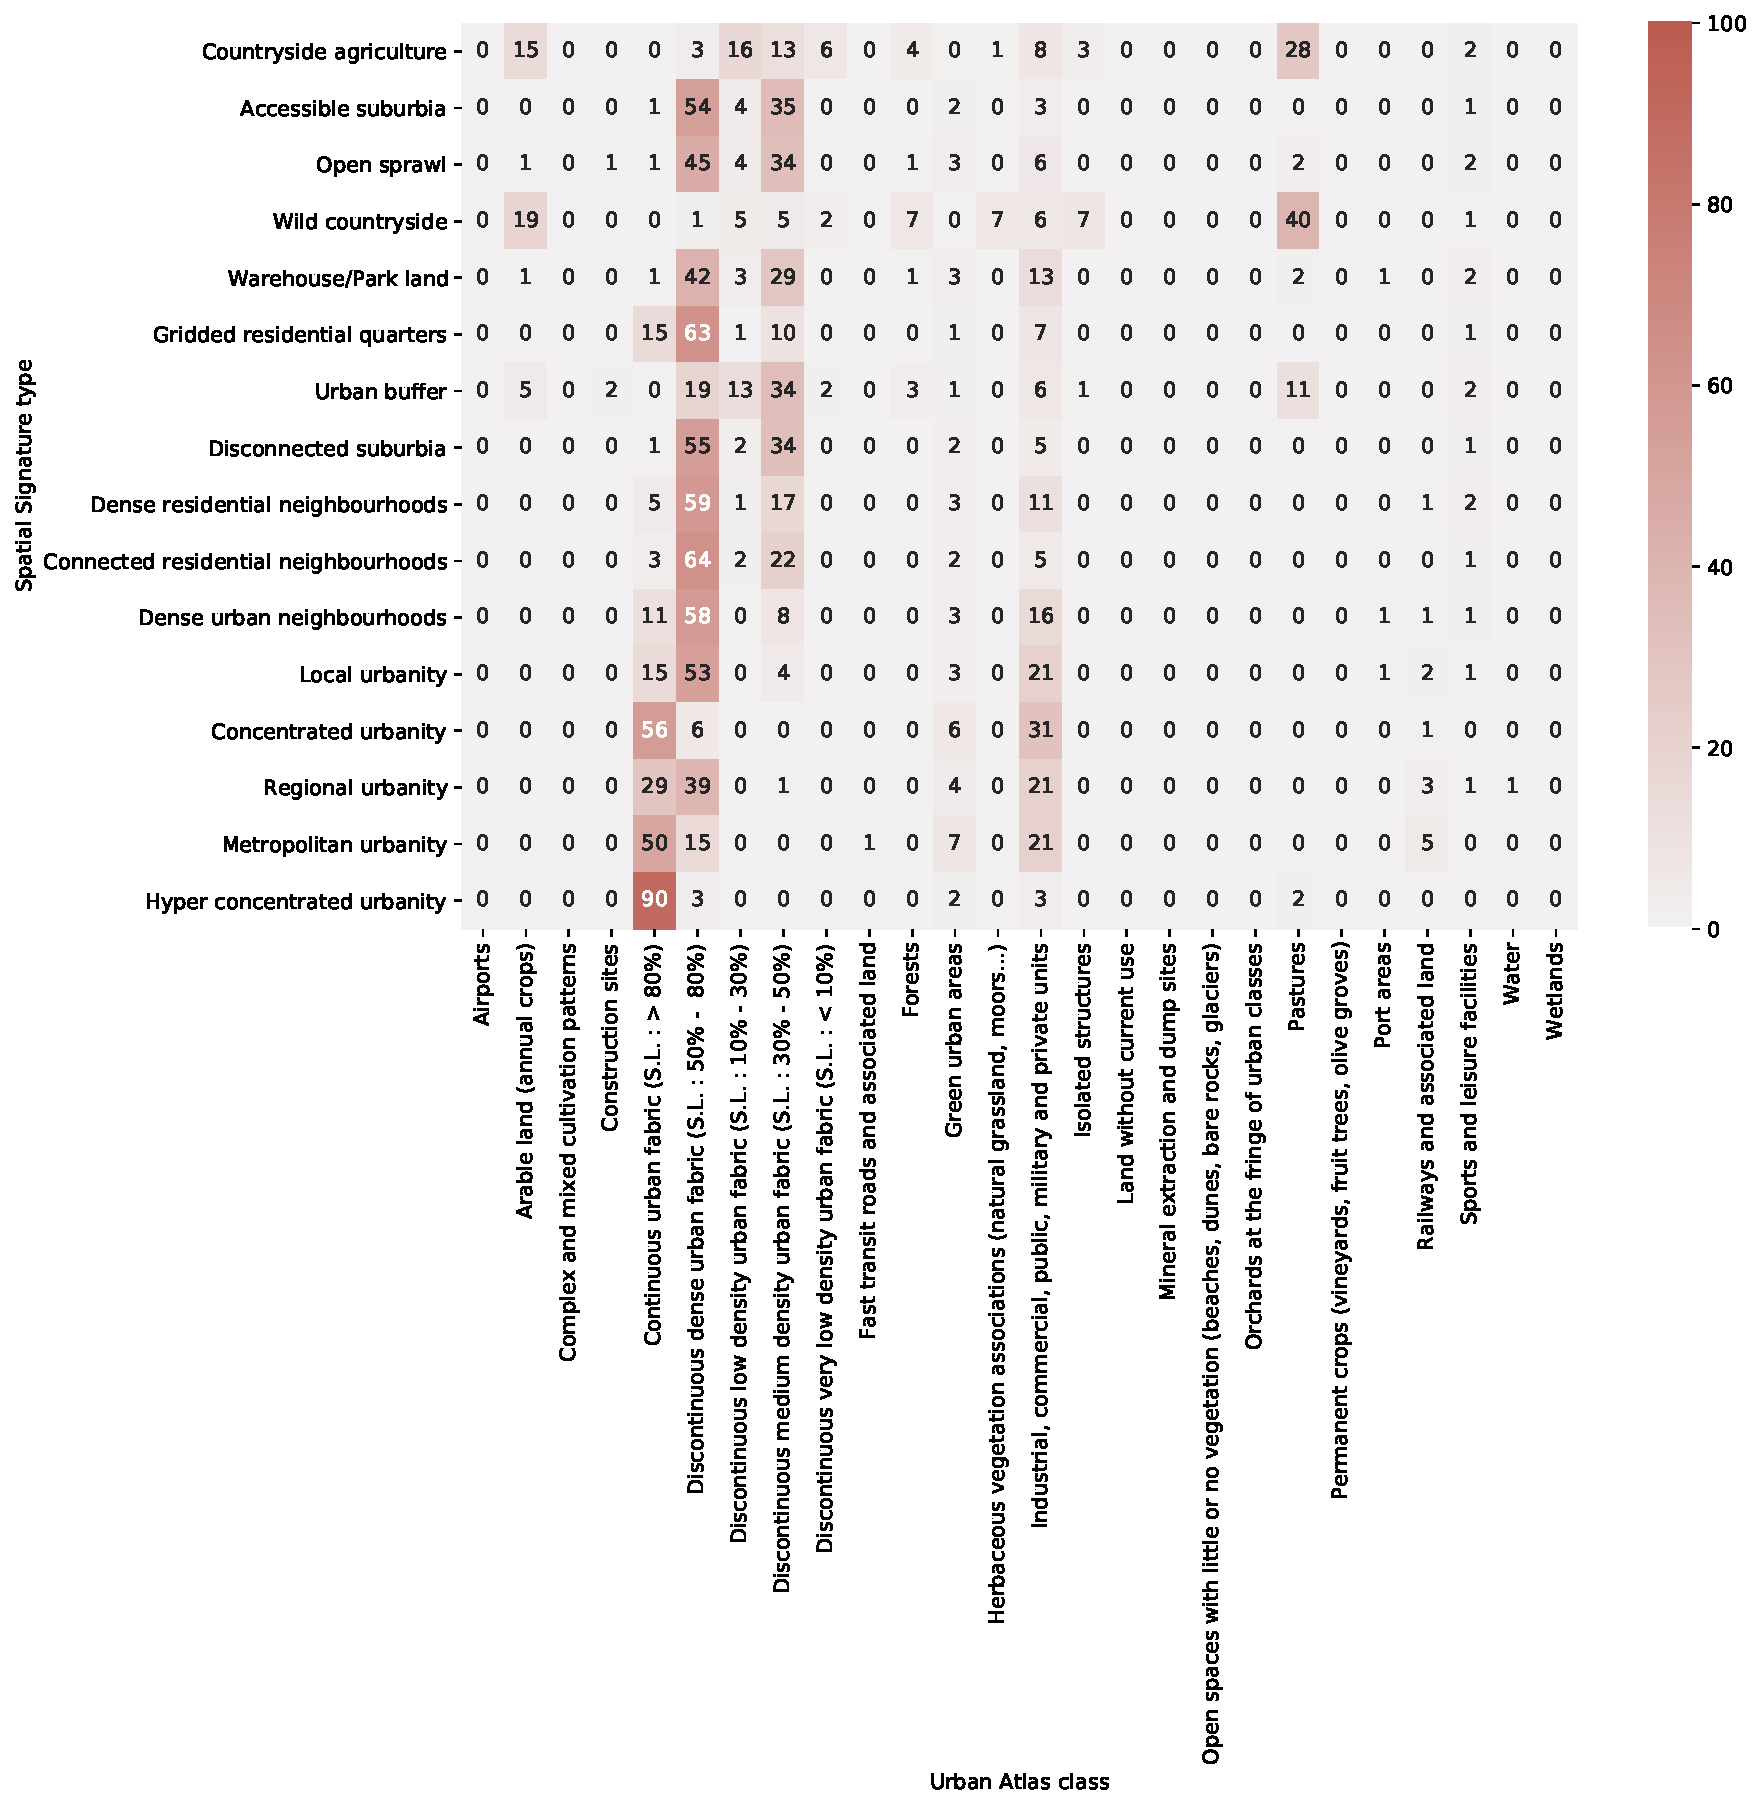
\includegraphics[width=\linewidth]{fig/crosstab_ua.pdf}
    \caption{Contingency table showing frequencies (in \%) of Urban Atlas classes within signature types.}
    \label{fig:crosstab_ua}
\end{figure}

\subsection*{Summary}
None of the comparisons shows more than a moderate association, but since none of the
validation datasets is aiming to capture the same conceptualization of space as spatial
signatures do, such a result is expected. The moderate association with both WorldPop
settlements patterns and MODUM is reassuring as both are conceptually closer to
signatures than the Urban Atlas (especially in their unsupervised design). Urban Atlas,
though very different in its aims and methods, still shows a measurable association,
which we interpret as sign that the key structural aspects forming cities are captured by both. The
validation exercise suggests that general patterns forming cities are shared among
signatures and existing typologies.




\section*{Usage Notes}

Released dataset is following the widespread standards for geographic data storage and
should not pose a challenge for researches wanting to reuse it. Due to the density of
signature geometry (resulting from the detailed ETCs), it may be needed to simplify the
geometry for smoother interactive experience on weaker machines.

Replication of the analysis optimally requires at least a single computational node with
large amount of RAM (100 GB+) due to the size of the input data and detail on which
signature characterization is computed. It is also recommended to revisit the state of
the development of related software packages, notably momepy, libpysal, tobler and
dask-geopandas as they may in the near future offer more efficient drop-in replacements
of the custom code used to produce this dataset.

\section*{Code availability}

The source code used to produce this dataset is openly available in a GitHub repository
at
\hyperlink{https://github.com/urbangrammarai/spatial\_signatures}{https://github.com/urbangrammarai/spatial\_signatures}
and in the form of a website on
\hyperlink{https://urbangrammarai.github.io}{https://urbangrammarai.github.io}.
Code is
organized in a series of Jupyter notebooks and have been executed within the darribas:gds\_env
Docker container, unless specified otherwise in the individual notebooks. The specific version
of the container is listed on top of each notebook.

\bibliography{refs}

\noindent LaTeX formats citations and references automatically using the bibliography
records in your .bib file, which you can edit via the project menu. Use the cite command
for an inline citation, e.g. \cite{Kaufman2020, Figueredo:2009dg, Babichev2002,
behringer2014manipulating}. For data citations of datasets uploaded to e.g.
\emph{figshare}, please use the \verb|howpublished| option in the bib entry to specify
the platform and the link, as in the \verb|Hao:gidmaps:2014| example in the sample
bibliography file. For journal articles, DOIs should be included for works in press that
do not yet have volume or page numbers. For other journal articles, DOIs should be
included uniformly for all articles or not at all. We recommend that you encode all DOIs
in your bibtex database as full URLs, e.g. https://doi.org/10.1007/s12110-009-9068-2.

\section*{Acknowledgements} (not compulsory)

Acknowledgements should be brief, and should not include thanks to anonymous referees
and editors, or effusive comments. Grant or contribution numbers may be acknowledged.

\section*{Author contributions statement}

Must include all authors, identified by initials, for example: A.A. conceived the
experiment(s), A.A. and B.A. conducted the experiment(s), C.A. and D.A. analysed the
results. All authors reviewed the manuscript.

\section*{Competing interests}

The authors declare no competing interests.

\section*{Figures \& Tables}

Figures, tables, and their legends, should be included at the end of the document.
Figures and tables can be referenced in \LaTeX{} using the ref command, e.g. Figure
\ref{fig:stream} and Table \ref{tab:example}.

Authors are encouraged to provide one or more tables that provide basic information on
the main ‘inputs’ to the study (e.g. samples, participants, or information sources) and
the main data outputs of the study. Tables in the manuscript should generally not be
used to present primary data (i.e. measurements). Tables containing primary data should
be submitted to an appropriate data repository.

Tables may be provided within the \LaTeX{} document or as separate files (tab-delimited
text or Excel files). Legends, where needed, should be included here. Generally, a Data
Descriptor should have fewer than ten Tables, but more may be allowed when needed.
Tables may be of any size, but only Tables which fit onto a single printed page will be
included in the PDF version of the article (up to a maximum of three).

Due to typesetting constraints, tables that do not fit onto a single A4 page cannot be
included in the PDF version of the article and will be made available in the online
version only. Any such tables must be labelled in the text as ‘Online-only’ tables and
numbered separately from the main table list e.g. ‘Table 1, Table 2, Online-only Table
1’ etc.

\begin{figure}[ht]
\centering
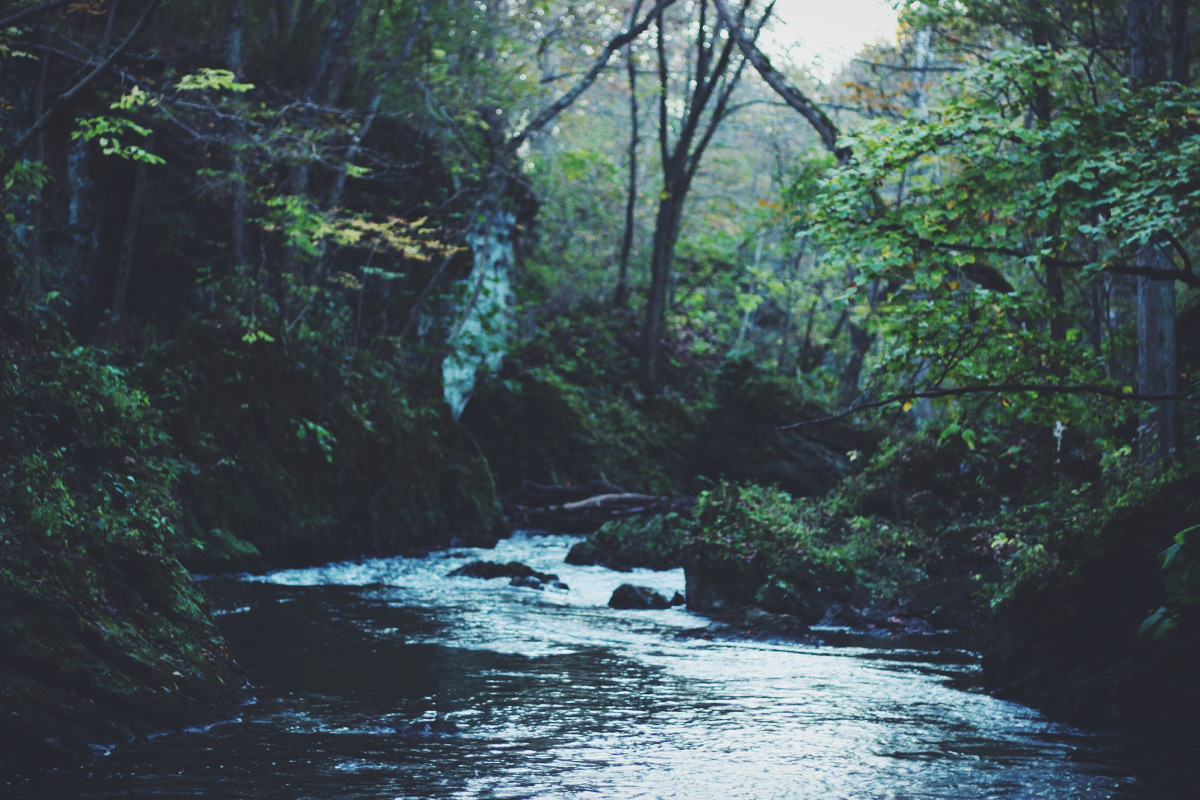
\includegraphics[width=\linewidth]{stream}
\caption{Legend (350 words max). Example legend text.}
\label{fig:stream}
\end{figure}

\begin{figure}
    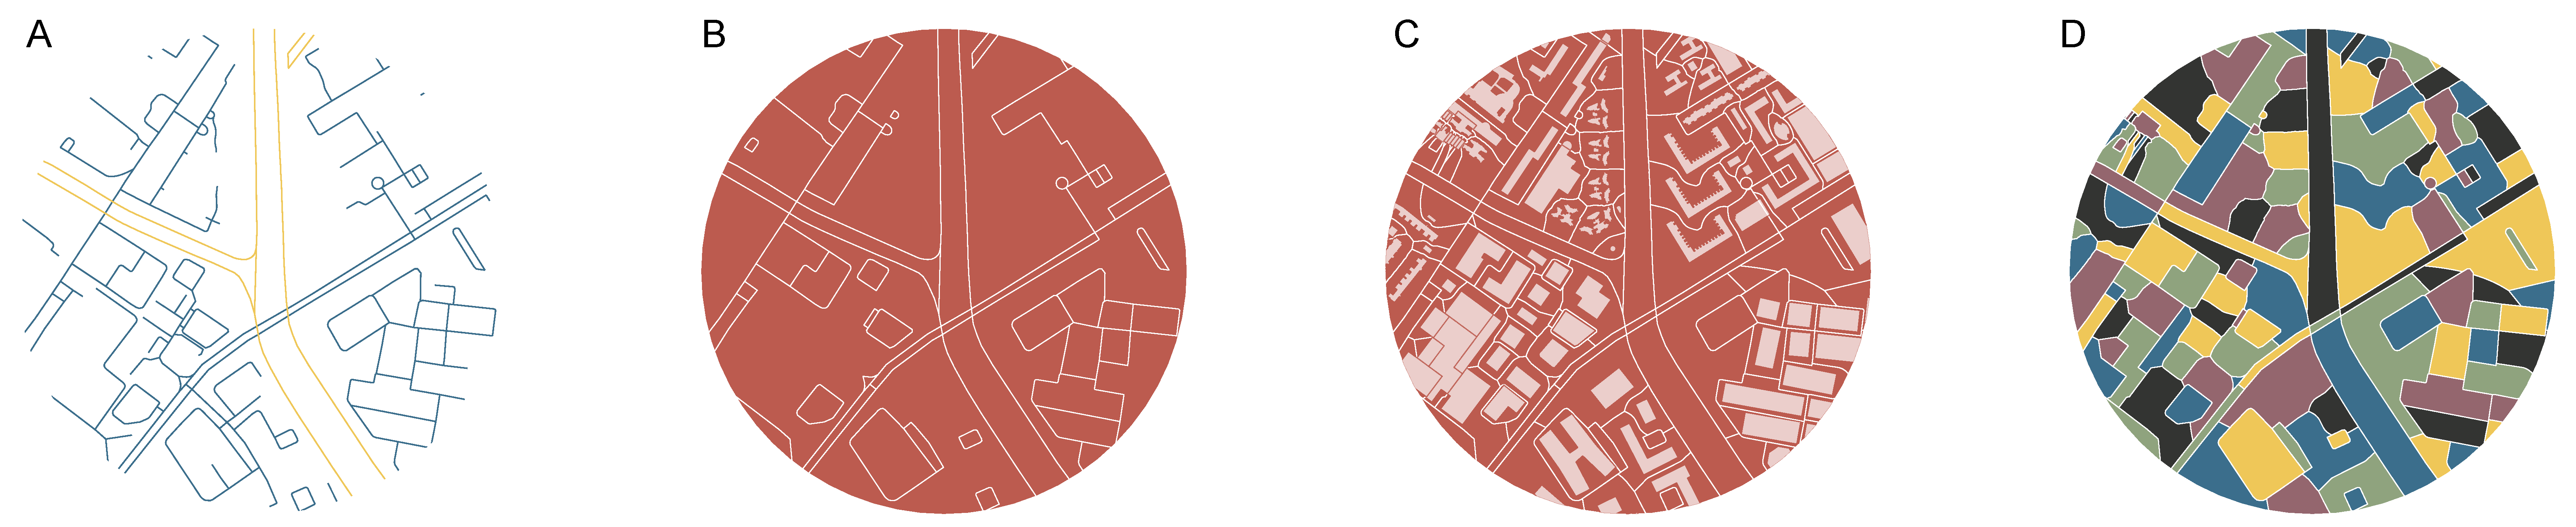
\includegraphics[width=\linewidth]{fig/et_diagram.pdf}
    \caption{Diagram illustrating the sequential steps leading to the delineation of
    enclosed tessellation. From a series of enclosing components, where blue are streets
    and yellow river banks (A), to enclosures (B), incorporation of buildings as anchors
    (C) to final tessellation cells (D).}
    \label{fig:et_diagram}
\end{figure}

\begin{table}[ht]
\centering
\begin{tabular}{|l|l|l|}
\hline
Condition & n & p \\
\hline
A & 5 & 0.1 \\
\hline
B & 10 & 0.01 \\
\hline
\end{tabular}
\caption{\label{tab:example}Legend (350 words max). Example legend text.}
\end{table}

\end{document}